\clearpage
\section{Critical algorithms}\label{sec:critical_algorithms}

This section discusses the progress made on the critical algorithms identified in the Data Reduction Library Specifications document \cite{DRLS}.

\begin{enumerate}
    \item[1.] Persistence correction (\ref{ssec:criticalpersistencecorrection})
    \begin{itemize}
        \item \textit{Reason at PDR}: Persistence is a major issue in modern IR detectors, and the determination of this pattern relies on observations previously done, which might arise from completely other observing runs and are therefore proprietary.
        \item \textit{Status at FDR}: The persistence correction algorithm will be developed by ESO, making the part in the Data Reduction Library non-critical.
        \item \textit{Prototype delivery}: None
    \end{itemize}
    \item[2.] Detector Masks (\ref{ssec:criticaldetetctormasks})
    \begin{itemize}
        \item \textit{Reason at PDR}: Reason unknown.
        \item \textit{Status at FDR}: Standard procedures apply, therefore not critical.
        \item \textit{Prototype delivery}: None.
    \end{itemize}
    \item[3.] Bad pixel determination (\ref{ssec:criticalbadpixeldetermination})
    \begin{itemize}
        \item \textit{Reason at PDR}: Reason unknown.
        \item \textit{Status at FDR}: Standard procedures apply, therefore not critical.
        \item \textit{Prototype delivery}: None.
    \end{itemize}
    \item[4.] Background subtraction (\ref{ssec:criticalbackgroundsubtraction})
    \begin{itemize}
        \item \textit{Reason at PDR}: A proper background correction is essential to ensure accurate photometric and spectroscopic analysis of the observed sources because observations in the mid-infrared are affected by the high sky and telescope background.
        \item \textit{Status at FDR}: Standard subtraction techniques (dithering, chopping and nodding) will be used, which not require prototying. More complex algorithms that would have required prototyping, e.g.
involving principal component analysis, have been ruled out since PDR.
        \item \textit{Prototype delivery}: None
    \end{itemize}
    \item[5a.] LSS Wavelength calibration and distortion correction (\ref{ssec:criticalwavelengthanddistortion})
    \begin{itemize}
        \item \textit{Reason at PDR}: A new algorithm is necessary for wavelength calibration and distortion correction for LSS.
        \item \textit{Status at FDR}: We will use the algorithm from PyReduce.
        \item \textit{Prototype delivery}: An adaptation of the PyReduce package.
    \end{itemize}
    \item[5b.] \ac{IFU} Wavelength calibration and distortion correction (\ref{ssec:criticalwavelengthanddistortion})
    \begin{itemize}
        \item \textit{Reason at PDR}: A new algorithm is necessary for wavelength calibration and distortion correction for IFU.
        \item \textit{Status at FDR}: We will use the same algorithm as CRIRES.
        \item \textit{Prototype delivery}: A script to call the CRIRES pipeline and example input/output files.
    \end{itemize}
    \item[6.] Telluric correction (\ref{ssec:criticaltelluriccorrection})
    \begin{itemize}
        \item \textit{Reason at PDR}: Telluric correction, i.e. the removal of absorption features arising in the Earth’s atmosphere, is a critical issue as the imprint of molecular species present in our air may vary on different timescales down to minutes due to changes in their composition and their amount.
        \item \textit{Status at FDR}: We either use molecfit or a telluric standard star. Both ways are well proven, and therefore we will not deliver a prototype
        \item \textit{Prototype delivery}: None.
    \end{itemize}
    \item[7.] Error propagation (\ref{ssec:criticalerrorpropagation})
    \begin{itemize}
        \item \textit{Reason at PDR}: Error propagation is important.
        \item \textit{Status at FDR}: The \ac{HDRL} provides standardized mechanisms for error propagation; prototyping is therefore not necessary.
        \item \textit{Prototype delivery}: None.
    \end{itemize}
    \item[8.] N-band image restoration (\ref{ssec:criticalnbandimagerestoration})
    \begin{itemize}
        \item \textit{Reason at PDR}: There is no standard algorithm for extended sources.
        \item \textit{Status at FDR}: Extended sources have been excluded, and the VISIR algorithm will be used for compact sources.
        \item \textit{Prototype delivery}: None.
    \end{itemize}
    \item[9.] LMS image and cube reconstruction (\ref{ssec:criticallmsimageandcubereconstruction})
    \begin{itemize}
        \item \textit{Reason at PDR}: Due to the width of the slices in the LM integral-field spectrograph of $20.7 mas$, the PSF is undersampled in the across-slice direction, and there is no known cube reconstruction algorithm.
        \item \textit{Status at FDR}: A prototype algorithm is implemented in Python.
        \item \textit{Prototype delivery}: Python package.
    \end{itemize}
    \item[10.] LMS data rate (\ref{ssec:criticallmsdatarate})
    \begin{itemize}
        \item \textit{Reason at PDR}: For very bright sources, the LM band spectrograph will have to operate with very short exposures, resulting in a high data rate of up to $1000 \mathrm{MiB}s^{-1}$ which may present a problem for the observatory pipeline which has to deal with the data in real time.
        \item \textit{Status at FDR}: The data rate is under control and does not require prototyping.
        \item \textit{Prototype delivery}: None.
    \end{itemize}
\end{enumerate}

The following additional critical algorithms were identified in the period between PDR and FDR:

\begin{enumerate}
    \item[11.] ADI algorithm (\ref{ssec:criticaladialgorithm})
    \begin{itemize}
        \item \textit{Reason at FDR}: Considering many of the science cases for METIS are focusing on direct imaging / high contrast imaging we deem it critical that we demonstrate that METIS-like data can be ADI-reduced without major issues.
        \item \textit{Status at FDR}: ADI algorithms for all HCI observing modes are known from literature, however considering many METIS science cases fall under HCI we demonstrate prototype ADI algorithms for the focal-plane and pupil-plane coronagraphs as well ADI+SDI for the partially undersampled \ac{IFU} with METIS-like simulated data.
        \item \textit{Prototype delivery}: Python package.
    \end{itemize}
\end{enumerate}

% Export these to individual files if they become too wordy
\subsection{Persistence correction}\label{ssec:criticalpersistencecorrection}
\label{sec_persistence_correction}
Persistence is a major issue in modern IR detectors, in particular in the Hawaii2RG devices (HgCdTe based).
This detector type also shows significant differences between the individual chips.
%The Aquarius (Si:As) seems to be less affected.
Fortunately, this pattern can be corrected via simple subtraction as a very first step.
However, since the determination of this pattern relies on observations previously done, this approach requires access to these data, which might arise from completely other observing runs and are therefore proprietory.
Therefore, the avoidance of persistence, i.e. a sophisticated planning / persistence management should be one of the major goals for the planning of the observations and the operational concept.
% It is not yet clear in how far a persistence correction is to be implemented in the pipelines.
%We therefore include that for the time being without detailed specification and assume this persistence maps to be external calibration input to the pipeline.


\TODO{Add figure from DRS? ``see Fig. 33 [taken from LBT website4 ]'' \url{https://sites.google.com/a/lbto.org/luci/instrument-characteristics/detector\#TOC-Persistence}
}

\TODO{Will have access to a HDRL function from ESO.
The interface is TBD.
Subtraction of persistence image as determined by ESO.
Need to reference ESO docs for this.
How does the scaling happen?
Is there an API endpoint for this?}


\subsection{Detector Masks}\label{ssec:criticaldetetctormasks}

In MATISSE the engineers created specific masks covering 32 pixels at the edge of the Aquarius detector, which was prone to crosstalk.
Crosstalk probably arises from the shared series buses in the detector readout electronics (see Figure on page 8 in~\cite{matisse_minutes}).
For the METIS detectors similar masks as in MATISSE are forseen in order to correct for crosstalk (cf. Polarion METIS-3093).
In~\cite{matisse_minutes}, the correction is described as follows:

\begin{displayquote}
Cross-talk correction is done in two steps using the masked pixels in the vertical direction, which are equivalent to two masked outputs.
\begin{itemize}
    \item Step 1 : The [w]hole line is corrected by an offset.
    \item Step 2 : Each pixel is corrected using the corresponding masked pixel in terms of raw
number in the two vertical masked outputs.
\end{itemize}
\end{displayquote}


\TODO{
Look into the MATISSE docs as to how this was done
Delivers a bias/dark/ron value?
Perhaps add Fig. 34 from DRS? Figure 34: Aquarius detector masks as realised in MATISSE ([RD11], courtesy of S. Mouzali).
Add Fig 35 from DRS? ``Figure 35: Correction for the crosstalk ([RD11], courtesy of S. Mouzali).''
}

\subsection{Bad pixel determination}\label{ssec:criticalbadpixeldetermination}

Bad pixels are an issue in any detector and have to be are monitored and stored.
This is usually done with the help of DARK and FLATFIELD frames.
Cold/hot pixels can be identified by using DARKS since they have pixel values which are far from an expected values (e.g.\ median value).
Non-linear pixels can be detected with illumination flats, that is, the detector is illuminated uniformly by a flatfield source.
Using  several exposure times / flux levels, non-linearities in pixels can be found by fitting polynomials to each  individual pixel.
We intend to introduce a bad pixel classification similar to the convention introduced in the X-Shooter Pipeline Manual (cf.\ Section 11.3 in~\cite{xshooter_manual}), adapted to our needs.

\TODO{
Surely every other instrument on planet earth has some sort of algo for this.
Need to determine the format of the bad pixel mask (bool?)
Take XSHOOTER as example ftp://ftp.eso.org/pub/dfs/pipelines/xshooter/xshoo-pipeline-manual-12.19.1.pdf
}

\subsection{Background subtraction}\label{ssec:criticalbackgroundsubtraction}
Observations in the mid-infrared are affected by the high sky background, the telescope background, and detector variations and non-linearities.
A proper background correction is thus essential to ensure accurate photometric and spectroscopic analysis of the observed sources.
As METIS will face an unprecedented level of complexity in the background subtraction due to (1) the high background dominated by the large number of warm mirrors, (2) the internal chopping, and (3) the complexities of nodding with an AO-corrected instrument, a dedicated research project has been started to better understand the origin of chop-residuals and to evaluate chop-only background removal strategies.
Hence, the dedicated pipeline algorithms will ultimately depend on the chosen strategy for each METIS detector, e.g.\ dithering, classical chop-nod, chop-counter-chop (in 1D or 2D), drift scanning.
%This is particularly relevant for the NQ bands where, for instance, the instability of the AQUARIUS detector response demands chopping at much higher frequencies.
More details on dedicated research project and the proposed strategies are given in the Calibration Plan \cite{METIS-calibration_plan} which serves as the base for the following.

\TODO{
N-band: Standard chop and nod using telescope chopper and internal nodder
See VISIR pipeline
}

\subsubsection{LM bands}
Small ($< 1000 \arcsec$) and slow (1 min timescale) dithered offsets of the field with respect to the LM IMG or \ac{IFU} detector are expected to be performed by the METIS-internal chopper mirror.
The pipeline shall determine the sky background from the dithered images and produce background maps without the sources and background-subtracted versions of the maps with the sources.
For In-field-dithering, this is done by determining a flux scaling factor for each ``dither'' position, aligning the exposures (by either using a 2d cross-correlation routine on bright sources or by using the offset values applied to the chopper), scaling the frames to a common median and removing objects by rejecting the highest and lowest pixels.
The remaining pixels are then averaged, or medianed, to produce the sky frame which is then scaled to match the median of the object frame before being subtracted.
The sky subtraction is further improved by following the previous steps to produce the combined image to locate all the sources.
Then the background frames are combined again while excluding the sources positions.
The best approach to determine the flux scaling factor of each dither exposure is yet to be determined (e.g.\ by median scaling or by a 2D/PCA approach based on \cite{Hunziker2018}).
The pipeline would also support sky subtraction using separate sky images for out-of-field dithering modes, i.e.\ when the observed field is crowded or full of extended emission.

\subsubsection{N bands}
To ensure proper background sampling at the longer wavelengths, small ($< 1000 \arcsec$) and fast ($\approx 10 \mathrm{Hz}$) chopping offsets of the field with respect to the N IMG detector are expected to be performed by the METIS- internal chopper mirror.
The chopping residuals from the previous step shall be corrected by nodding the telescope to a different position and repeating the same chopping procedure.
The chopping and nodding sequence is expected to follow what is currently being done with VISIR.
The pipeline shall determine the sky background from the chopped and nodded images and produce background maps without the sources and background-subtracted versions of the maps with the sources.
For each nodding cycle the subsequent chop-cycle frames are subtracted from each other (mean of on-source frames minus mean of off-source frames) resulting in a single chop-difference frame, i.e. nod half-cycle frame.
Then for subsequent nodding cycles the nod half-cycle frames are subtracted from each other resulting in a nod-difference frame.
The mean of all nod-difference frames is the final background-subtracted image.
Additionally, the optimal extraction (PSF-weighting) will be used to subtract the positive/negative source images from the final background-subtract image (2/3/4 depending on the relative chopping/nodding directions) to produce a single stacked image of the sources of interest.

\subsection{Wavelength calibration and distortion correction}\label{ssec:criticalwavelengthanddistortion}

Pyreduce, will be described by Nadeen
IMG modes are not critical, see recipes

\subsection{Telluric correction}\label{ssec:criticaltelluriccorrection}
Telluric correction, i.e. the removal of absorption features arising in the Earth's atmosphere, is a critical issue as the imprint of molecular species present in our air may vary on different timescales down to minutes due to changes in their composition and their amount. In particular the \ac{MIR} range is affected (see App~\ref{app:atmo_trans}).\\
There are two well established ways to correct for these absorptions:
\begin{itemize}
    \item \textit{Classical approach}: A telluric standard star (\ac{TSS}) spectrum is taken ideally directly before/after the science observations at the same airmass. This \ac{TSS}-spectrum is processed in the same way as the science spectrum (except the absolute flux calibration) and finally its continuum is normalised to unity. In addition, a model of this specific \ac{TSS} spectrum is used to remove intrinsic spectral features. The remaining normalised spectrum (ideally) only contains the fingerprint of the Earth's atmospheric absorptions and can be used for the telluric correction. In case the model spectrum also contains absolute flux values, this star could also be appropriate for the absolute flux calibration.
    \item \textit{Modelling approach}: In the last years a new method has evolved which is based on radiative transfer modelling of the Earth's atmosphere (\cite{mf1, mf2, molecfit}\footnote{\url{https://www.eso.org/sci/software/pipelines/skytools/molecfit}}). A model of the Earth's atmosphere in combination with a radiative transfer model and a molecular line list containing lines of various species is used to determine the transmission of the Earth's atmosphere at the time of observations by fitting specific molecular absorption features in the science spectra. The best-fit transmission function is finally used for the telluric correction.
\end{itemize}
These two methods can also be combined in the way that the modelling approach is applied to a \ac{TSS} spectrum, and the resulting transmission function is then applied to the science spectrum. This combination is specifically useful if the science target continuum is too weak to use the absorptions for a fit.\\
For the \ac{METIS} pipelines we intend to incorporate both ways (including their combination). A detailed description is given in Section~\ref{ssec:tellcorr}. As both methods are well established, we deem a dedicated prototyping not necessary.

\subsection{Error propagation}\label{ssec:criticalerrorpropagation}

HDRL functions do error propogation. Look into docs for these. 
Understand how HDRL does this and then copy it.

\subsection{N-band image restoration}\label{ssec:criticalnbandimagerestoration}

Chop-nod inversion and stacking
Look at how VISIR does this
Need to look at sub-pixel chop shifts, and whether the images need to be resampled
Plate scale distortions are not really a issue, because we only care about compact objects

\subsection{LMS image and cube reconstruction}\label{ssec:criticallmsimageandcubereconstruction}

Completely open and a bit of a beast. 
Help from Linz?
Drizzling from HST?

\subsection{LMS data rate}\label{ssec:criticallmsdatarate}

\TODO{Placeholder text below is based on the PDR DRS and needs to be updated. See data rate document. Add arguments to make this a non-.}
\label{ssec:lms_data_rate}

For very bright sources, the LM band spectrograph will have to operate
with very short exposures, resulting in a high data rate of up to
$1000\,\mathrm{MiB\,s^{-1}}$ (cf.~Table~\ref{tab:data_rates}). This
high data rate may present a problem for the observatory pipeline
which has to deal with the data in real time.  The observatory
pipeline does not have to perform a full data reduction as described
in Sect.~\ref{sssec:lms_sci_process}, but merely compute a number of
quality control parameters to assess the quality of the data. In the
course of the development of the observatory recipe dealing with LMS
science data, the question of data rates will need to be
considered. If necessary, the performance of the recipe may need to be
reduced if a high data stream is to be expected. Another option might
be to compute QC parameters only on a subset of incoming frames.


% Additional critical algos
\subsection{ADI algorithm}\label{ssec:criticaladialgorithm}
Considering many of the science cases for METIS are focusing on direct imaging / high contrast imaging we deem it critical that we demonstrate that METIS-like data can be ADI-reduced without major issues.
ADI reduction with focal plane and pupil plane coronagraphs, in addition to ADI+SDI with the IFU (partially spatially undersampled with an additional spectral dimension) is therefore demonstrated.
It is recognized that the required techniques are already known from earlier publications of data collected with high contrast imagers and AO-fed IFUs.
This study allows the PIP team to become more familiar with them and to present prototype algorithms in a centralized location.

\subsubsection{Generation of representative set of IMG\_LM data: planetary system}
Using a combination of the HEEPS code and the ScopeSim code with the METIS package we have performed simulations of a star and a point source companion in order to test critical algorithms for high contrast imaging on simulated data of METIS.
Using the HEEPS code we simulate a sequence of up to 12000 PSFs of an unresolved star behind the RAVC coronagraph and of an unresolved companion sufficiently far away from the coronagraph to be considered off-axis, with each PSF corresponding with an integration time of 300 milliseconds for a total of 3600 seconds of observing time. Each PSF is generated with a (SCAO-only) wavefront sampled every 300 ms (comparable to the coherence time t0 at L-band), thereby effectively time sampling the atmospheric wavefront aberrations. Both PSFs are scaled to the magnitude of the parent star ($L=3.5$). For this demonstration we use a time sequence of 12000 PSFs but will apply some windowing and temporal binning to increase execution speed on a laptop. 
The two PSFs are combined together with an offset of 100 mas, an additional delta magnitude ($\Delta L=7.7$) for the companion and field rotation over 1 hour (corresponding with 30 degrees change in position angle). The system could be described at Beta Pic b orbiting at 100 mas around its host star. A second source is added at opposite position angle to see the symmetry of the reduction (of use for the APP coronagraph which only has one dark hole). This combined source is fed into ScopeSim as a fits file with the WCS information conveying the spatial extent. The coronagraphic transmissions are transferred to ScopeSim as well during this process.
In the ScopeSim step the instrumental noise and background expected from both METIS and ELT is injected and the source flux reduced according to system transmission. 
After these processing steps we are left with a large 3D cube of a star (x, y, time) with two planets undergoing field rotation which we use for the ADI processing step using the VIP\_HCI package. For this example, the output images have been truncated to 201x201 pixels and the images have been binned to 30 seconds exposure time ($N_\mathrm{bin}=100$) to further reduce execution time.
\subsubsection{Demonstration of ADI algorithm on simulated IMG\_LM data}
The most basic PSF subtraction of VIP\_HCI is the standard ADI algorithm from Marois et al 2006, where the median of the cube is first subtracted and in a second step optimally-scaled time-localized medians are subtracted in annular rings. Afterwards each image in the cube is derotated with the known position angle. Subsequently the derotated and PSF subtracted images are averaged to give a final stacked version. When the second annular optimized subtraction step is skipped this procedure is equal to the one described in the PIP Spec.
For the IFU, this ADI procedure can similarly be followed for each wavelength in the reduced cubes. In VIP\_HCI it is possible to do a two-step (first ADI then SDI) or single-step reduction, in which rescaled images from other wavelength slices are used to provide additional PSF reference material.
Example output images for ADI reduction for LM RAVC data.


\begin{figure}[!ht]
  \centering
  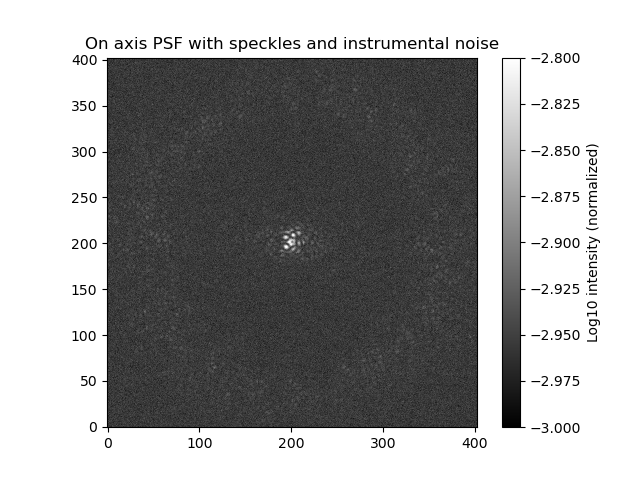
\includegraphics[width=0.6\textwidth]{./figures/onaxis_psf.png}
  \caption{On-axis coronagraphic PSF with instrumental noise injected and with corrected atmospheric turbulence. The circular control region from the AO system is clearly visible.}
  %\label{fig:metis_l}
\end{figure}
\begin{figure}[!ht]
  \centering
  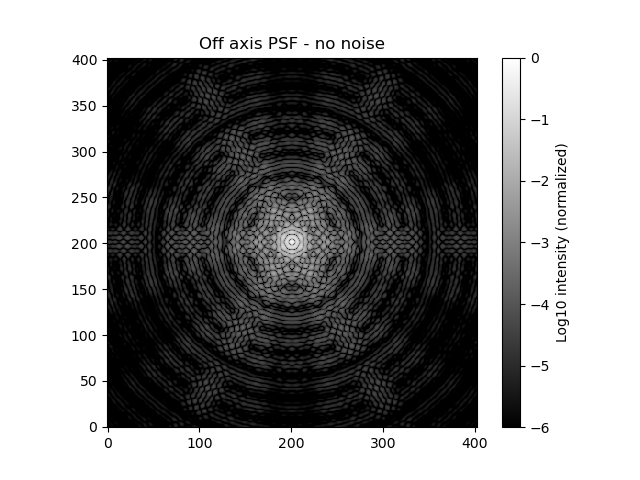
\includegraphics[width=0.6\textwidth]{./figures/offaxis_psf.png}
  \caption{Off-axis PSF without instrumental noise.}
  %\label{fig:metis_l}
\end{figure}

\begin{figure}[!ht]
  \centering
  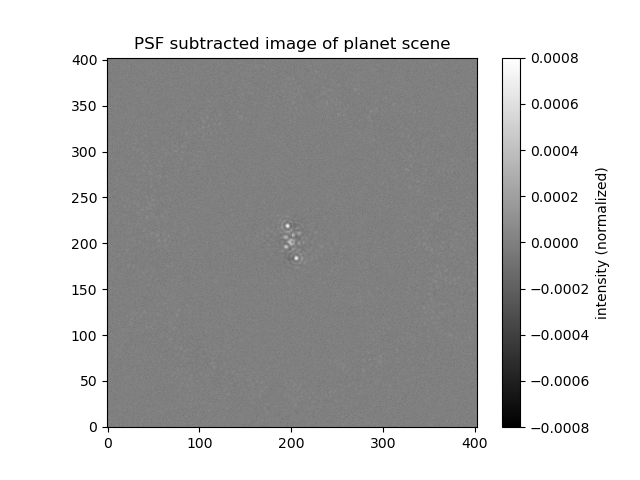
\includegraphics[width=0.6\textwidth]{./figures/adi_meansub.png}
  \caption{Single frame of image stack with mean PSF subtracted.}
  %\label{fig:metis_l}
\end{figure}

\begin{figure}[!ht]
  \centering
  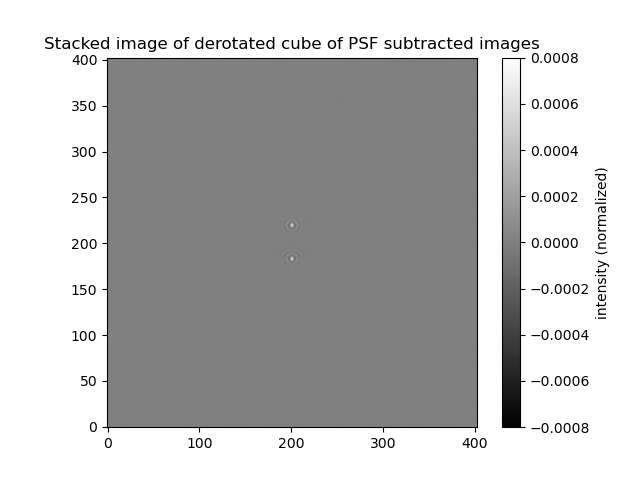
\includegraphics[width=0.6\textwidth]{./figures/adi_derotstack.png}
  \caption{Derotated stack of ADI reduced images.}
  %\label{fig:metis_l}
\end{figure}

Additionally, the contrast curves can be extracted (raw contrast over time-averaged cube, 5 sigma contrast after ADI processing). Please note that the plotted contrast is dependent on the assumptions made for this demonstration (SCAO-only effects, no additional jitter / pupil drifts / no residual atmospheric dispersion, 120 binned frames with each 100 frames of 0.3s integration time, 30 degrees image rotation). 
Injection and retrieval of point sources of known intensity is performed to calculate the efficiency or throughput of the ADI post-processing technique. Closer to the star the same amount of position angle movement will be seen as an increasingly smaller physical movement. Therefore, self-subtraction of a point source signal will be more pronounced and increased losses are seen close to the star. The following plot shows the post-processing only component of the ADI reduction losses. The radial coronagraphic throughput losses due to partial suppression of off-axis sources will be provided separately (and is not included in these sensitivity plots for this example).



Following the SNR definitions of Mawet et al 2014 the noise is calculated in annular rings and corrected for the relatively low number of effective samples. A 5-sigma sensitivity curve is produced by injection and retrieval of sources. In addition, a post-ADI SNR map is generated. Note that the two injection planets are so bright that an unmasked SNR map gives an underestimated SNR as their presence strongly alters the local noise estimate. Nonetheless they are both recognized as significant detections.

\begin{figure}[!ht]
  \centering
  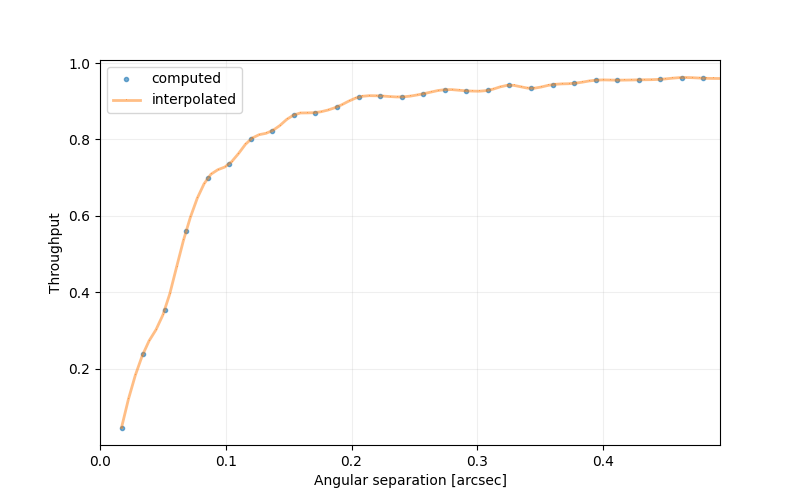
\includegraphics[width=0.6\textwidth]{./figures/adi_throughput.png}
  \caption{Efficiency of ADI algorithm in retrieving inserted point sources as a function of angular separation.}
  %\label{fig:metis_l}
\end{figure}

\begin{figure}[!ht]
  \centering
  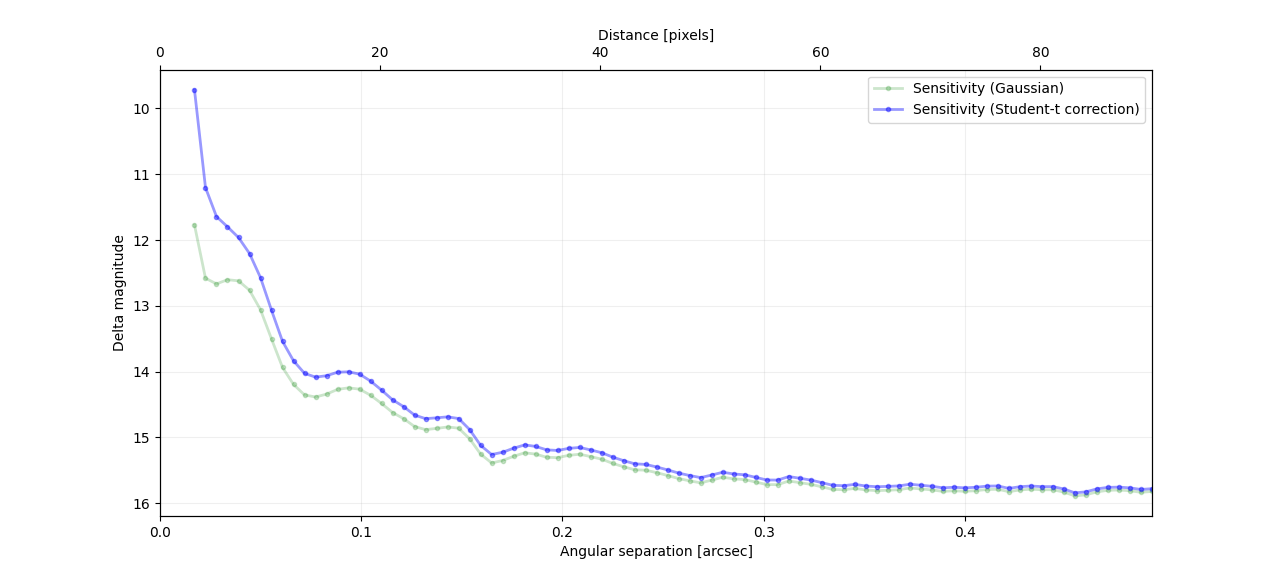
\includegraphics[width=0.6\textwidth]{./figures/adi_contrast.png}
  \caption{Achievable contrast for the $L=3.5$ target in 1 hour integration time as a function of angular separation.}
  %\label{fig:metis_l}
\end{figure}

\begin{figure}[!ht]
  \centering
  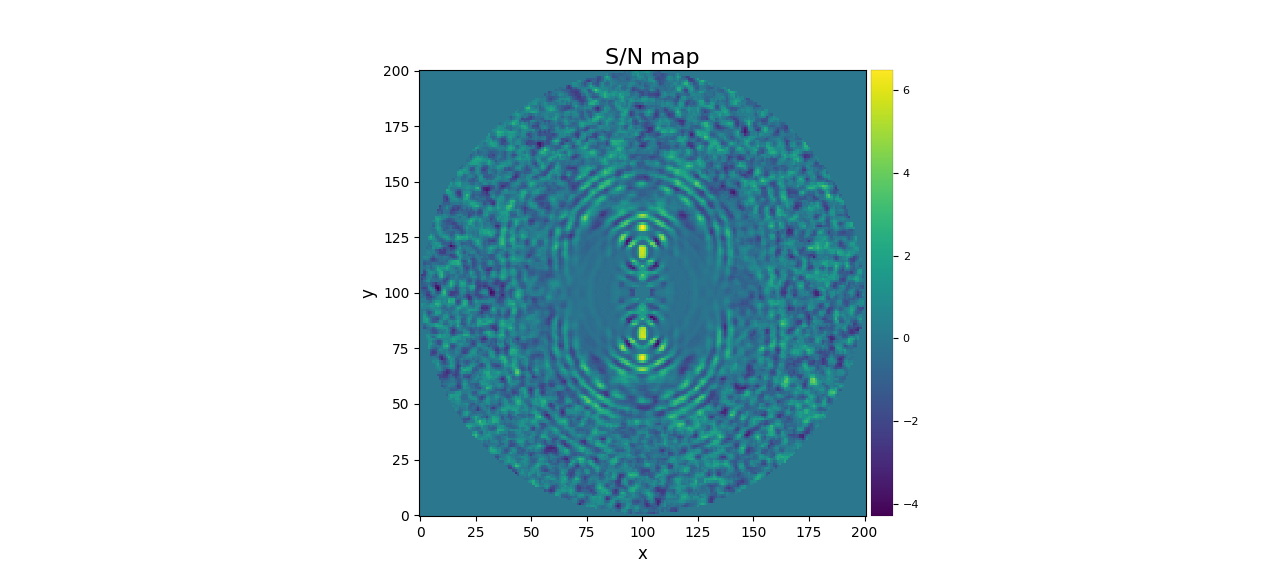
\includegraphics[width=0.6\textwidth]{./figures/adi_snrmap.png}
  \caption{Two dimensional ADI map of post ADI signal to noise of point sources. Two point sources that were inserted at 100 mas are seen.}
  %\label{fig:metis_l}
\end{figure}

\subsubsection{Generation of representative set of IFU data}

To demonstrate the ADI/SDI reduction of an IFU dataset which contains spatial, temporal and spectral information we first generate a METIS IFU HCI dataset of 12000 frames by 267 by 267 pixels and Z spectral bins. Each frame corresponds with an exposure time of 0.3 seconds, with a total integration time of 1 hour.  
We generate PSFs with the HEEPS python code in L band with the RAVC coronagraph at a pixel scale of 8.2 by 8.2 mas. At a central wavelength of 3.8 micron this corresponds to approximately 100 by 100 lambda/D. This data is FFT interpolated with VIP\_HCI with a scaling factor to generate 1600 spectral bins in a wavelength range of X micron at a wavelength of X micron. 
As the METIS IFU projected on-sky has rectangular pixels we average the data in one dimension to get a pixel scale of 8.2 by 24.6 mas (note actual scale is close to 8.2 x 21 mas). The sum of all flux is set to be equal to the total photons of the star in L-band.
To go back to square pixels, we duplicate the undersampled axis. We inject noise according to the shot noise of the source, sky background and detector read noise with a single resolution element spanning about x by x pixels, while also using a binning factor of X spectrally and 100 temporally to reduce memory consumption.



 


\subsubsection{Demonstration of ADI+SDI algorithm on IFU data}


This dataset is used together with an array containing a set of position angles given 1 hour of sky rotation and an array containing the wavelengths of the spectral axis to perform a median PSF subtraction technique using VIP\_HCI on the generated data. This is a two-step process where first for each timestep all spectral slices are rescaled to be on the same lambda/D grid. Then the median of the cube in the spectral dimension is subtracted. This is repeated for every timestep to give a time varying array of residuals. For this array the median in time is also calculated and subtracted. Afterwards the residuals are derotated and stacked and analysed yielding the following 5 sigma performance curves. 

[insert images of IFU ADI+SDI data reduction]
